\section{Results}
\label{sec:results}

% Test-set results in the main text, validation results in the appendix. Before each experiment,
% state the claim it tests. Every number is a paired change over seeds 0-4 (mean, sample SD, verdict).
% Tables are generated by src/component/analyze_results.py and stage2_results.py (--split test);
% the test tables appear here once they are on main.

\subsection{Synthetic images with pretrained classifiers}
\label{sec:results-pretrained}
\todo{claim and numbers: class-prompt images vs real-only and vs RandAugment, pretrained, by budget (test)}

\resulttable{stage1_pretrained_test_accuracy_sd_prompt}
\resulttable{stage1_pretrained_test_accuracy_vs_randaugment}

\subsection{The sign flip with initialization}
\label{sec:results-flip}
\todo{claim and numbers: the same images lose to RandAugment from random initialization; ResNet-50,
ViT-B/16 and ConvNeXt-T, every seed (test)}

\resulttable{stage1_scratch_test_accuracy_vs_randaugment}
\resulttable{stage2_convnext_pretrained_test}
\resulttable{stage2_convnext_scratch_test}

\subsection{More generated images per real image}
\label{sec:results-ratio}
\todo{claim and numbers: 1:1, 2:1, 5:1; all 36 ratio-vs-real comparisons are gains on validation and
test; from scratch 5:1 beats RandAugment in 3 of 4 cells}

\resulttable{stage2_ratio_pretrained_test}
\resulttable{stage2_ratio_scratch_test}

\subsection{Stronger conventional augmentation}
\label{sec:results-augment}
\todo{claim and numbers: Mixup, CutMix, TrivialAugment, AutoAugment and AugMix alone and combined
with class-prompt images, from random initialization; augmentation seeds 1-4 are still running}

\resulttable{stage2_mixing_pretrained_test}
\resulttable{stage2_mixing_scratch_test}
% TODO: table for the policy and stacked conditions (runs/augment-scratch) once all seeds are in.

\subsection{A generator trained only on the real images}
\label{sec:results-gan}
\todo{table of the GAN set at 50 images per class, both initializations, test, 5 seeds}
% Test-set paired changes, GAN minus real-only, mean over seeds 0-4 (from runs/gan-*):
%   pretrained ResNet-50 -2.97, ViT-B/16 -3.50 (0/5 seeds positive);
%   scratch ResNet-50 +4.59, ViT-B/16 +3.89 (5/5 positive).
%   Scratch ViT-B/16: GAN minus SD class prompts +0.65 (5/5); scratch ResNet-50: -4.06 (0/5).
% Generate the table with a script before quoting these numbers in text.

\subsection{Does generator quality predict usefulness?}
\label{sec:pool-utility}
% Moved from the report (validation scores; check against the test scores before submission).
FID and Improved Precision \& Recall describe a generated set without training on it. To test whether they
predict which set helps more, we compare the generated sets of each budget: SD class prompts, the LoRA set
of that budget and the SD img2img edits of the budget's own real images (5 to 50 images per class; the full
set has the first two). Every pair of sets is compared within each budget, classifier and initialization
(52 comparisons). A comparison agrees when the set a measure rates better also gives the larger paired gain
over real-only, averaged over the seeds both sets share (seeds 0--2). Comparing within a budget is
necessary: both FID and the gain shrink as the budget grows, so across budgets any measure would appear to
predict the gain through the budget alone.

Two details of the measurement matter. First, the img2img edits and the LoRA adapter are made from the
budget's own real images, and a reference sample drawn from the whole training pool contains some of them
(6 of 500 reference images at 5 images per class, up to 557 of 5,000 at 50), which would flatter those sets.
From 5 to 50 images per class, all three sets are therefore scored against a reference that leaves the
budget's images out. This moves the img2img FID by at most 1.5 (94.1 to 95.5 at 5 images per class) and
changes no conclusion below. Second, the comparisons are not independent: a measure rates each pair of
sets once per budget, and the two classifiers and two initializations of that budget share the verdict.
Where a pair's verdict is the same at every budget, the measure agrees exactly where the favoured set wins,
so we test a measure only on the pairs whose verdict changes between budgets. FID minus the
real-versus-real floor is not a separate measure, since the sets of a budget share the floor.

Table~\ref{tab:pool-utility} and Figure~\ref{fig:pool-utility} give the result. The usefulness of the three
sets follows one order. The class-prompt set gives a larger gain than the LoRA set in 17 of 20 comparisons
(all 10 with pretrained classifiers, in 29 of 30 seed pairs) and than the img2img set in all 16, and the
LoRA set a larger gain than the img2img set in 13 of 16. FID and recall rank the sets in the opposite order
at every budget: img2img first, then LoRA, then class prompts. They pick the more useful set in only 6 of 52
comparisons, the few where the order of usefulness is reversed: the LoRA set ahead of the class-prompt set
in three cells from random initialization (ResNet-50 at 20 images per class, and both classifiers on the
full set, by 2.4 and 2.1 points), and the img2img set ahead of the LoRA set in three pretrained cells at 20
and 50 images per class. Because their verdict never changes, we give them no $p$-value, but the pattern is
plain: the sets that these measures rate closest to the real data help least.

Precision rates the class-prompt set above both others at every budget and so agrees in 42 of 52
comparisons, but that count mostly restates that the class-prompt set wins. The one pair whose precision
verdict changes between budgets is LoRA against img2img (LoRA ahead at 10 and 20 images per class, img2img
at 5 and 50, by 0.01 to 0.02), and there precision picks the more useful set in 9 of 16 comparisons, at
chance ($p = 0.80$). The third set thus answers the question that two sets left open: none of the three
measures predicts which generated set will help beyond the advantage of the class-prompt set.

The order of usefulness matches how far each set is from the budget's own real images. The class-prompt
images never see them, the LoRA adapter is fitted to them, and the img2img edits keep their layout and
colours. One explanation consistent with this order, which we have not tested directly, is that in the
scarce-data setting a generated set helps by adding what the few real images lack, while FID and recall
reward closeness to the real data and so rank the sets the wrong way round. The order also
holds from random initialization, where the class-prompt set is ahead of the img2img set in all 8
comparisons and by 3.4 and 5.7 points for ResNet-50 at 20 and 50 images per class.
% TODO: add the GAN set at 50 images per class (FID 25.9 vs its own training images; measure it
% with the same reference and floor as the other sets before comparing).

\resulttable{pool_utility_summary}

\begin{figure}[H]
\centering
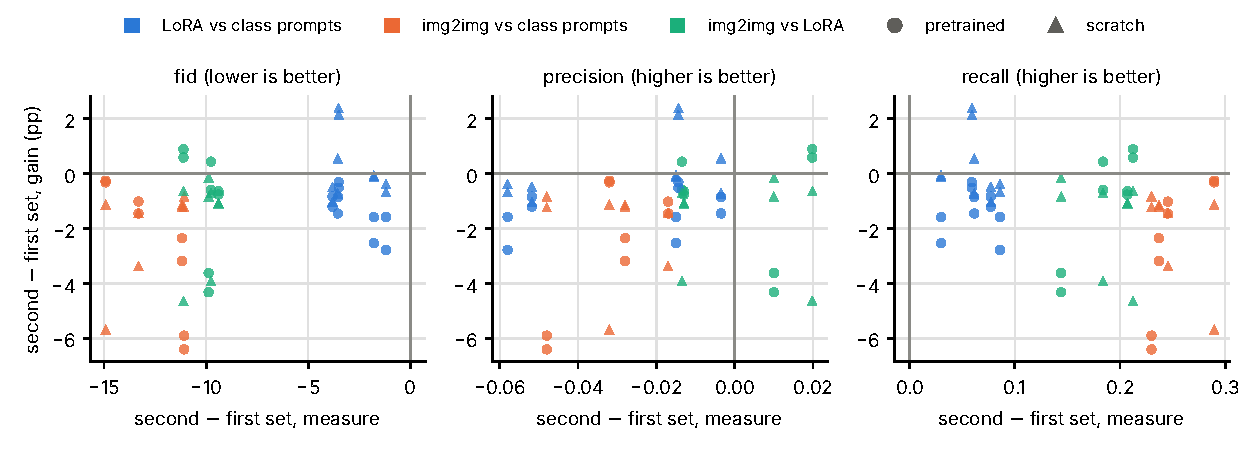
\includegraphics[width=\textwidth]{pool_utility_measure_vs_gain.pdf}
\caption{For each pair of generated sets (colour), the second set minus the first, in each quality
measure (x) and in the paired gain over real-only (y), one point per budget and classifier; circles:
pretrained, triangles: random initialization. A measure that predicts usefulness puts the points in the two
quadrants where its sign matches the gain's (for FID, lower is better, so the upper-left and lower-right
quadrants). The scores at 5 to 50 images per class use a reference without the budget's own images.}
\label{fig:pool-utility}
\end{figure}

\subsection{Why the effect flips with initialization}
\label{sec:sign-flip}
% Moved from the report (validation and training images only).
SD class-prompt images raise the accuracy of ImageNet-pretrained classifiers at every budget but lose to
RandAugment for randomly initialized ones at most budgets. We tested two explanations on validation and
training images only.

\paragraph{Diversity and per-class distance do not explain it.}
For each class we compared 50 generated with 50 real training images in Inception feature space:
Improved Precision and Recall within the class, the spread of the generated images relative to the real
ones, and the distance between the two class means. The generated images are realistic but narrow
(mean per-class precision 0.73, recall 0.26, spread 0.86 of the real class). None of these measures
predicts the per-class recall change of SD over real-only at 5 images per class, for either
initialization ($|\rho| \le 0.19$, no permutation $p$ below 0.05 over the 100 classes). Over all 60
correlations we computed, the only ones that survive a Holm correction concern the change
of scratch ResNet-50 over RandAugment (precision $\rho = +0.36$, Holm $p = 0.024$), and they come from
RandAugment's own per-class gain ($\rho = -0.40$, Holm $p = 0.006$), not from SD. With 100 classes a
correlation must exceed about 0.20 to reach $p < 0.05$, and only true correlations of about 0.28 or more
are detected with 80\% power, so weaker per-class effects may be missed.

\paragraph{A real-only classifier recognises the generated images less well from scratch.}
Table~\ref{tab:synthetic-accuracy} gives the accuracy of classifiers trained on real images only on
5{,}000 generated images (50 per class), next to their accuracy on the real validation images. Pretrained
classifiers recognise the generated images almost as well as real ones (93--97\% of their validation
accuracy on the full training set, 99\% at 5 images per class). Classifiers trained from scratch lose
about 9 points on them even with the full training set (79--83\%). The generated images are faithful to
their class, which answers how good the generation is, but they lie in a region that features learned
from CIFAR-100 alone cover less well. A pretrained backbone bridges this shift; a network trained from
scratch must learn both distributions from the same few images, and the generated images help it less
than RandAugment's perturbations of the real ones. Per class, the accuracy of the full-data real-only
classifiers on the generated images is weakly but consistently related to the gain of SD over real-only
($\rho = 0.15$--$0.29$ over the four classifiers, none significant after the Holm correction). For
pretrained classifiers this relation is specific to SD ($\rho = 0.06$--$0.08$ for RandAugment); from scratch
it is about as strong for RandAugment ($\rho = 0.16$--$0.19$), so there it partly reflects how easy a class
is. Because the per-class relations are weak, the shift appears to be a property of the generated set as a
whole rather than of particular classes.

\begin{table}[H]
\centering
\small
\caption{Accuracy (\%) of real-only classifiers (seed 0) on the real validation images and on 5{,}000 SD
class-prompt images (50 per class), and the second as a share of the first. At 5 images per class the
scratch classifiers are close to chance (1\%), so their ratios are noisy.}
\label{tab:synthetic-accuracy}
\begin{tabular}{llrrrr}
\toprule
Initialization & Model & Images/class & Real val. & Generated & Ratio \\
\midrule
Pretrained & ResNet-50 & full & 84.22 & 78.24 & 0.93 \\
Pretrained & ViT-B/16  & full & 88.62 & 85.84 & 0.97 \\
Scratch    & ResNet-50 & full & 54.44 & 45.14 & 0.83 \\
Scratch    & ViT-B/16  & full & 43.72 & 34.44 & 0.79 \\
\midrule
Pretrained & ResNet-50 & 5 & 35.66 & 35.46 & 0.99 \\
Pretrained & ViT-B/16  & 5 & 45.14 & 44.78 & 0.99 \\
Scratch    & ResNet-50 & 5 & 8.60  & 6.00  & 0.70 \\
Scratch    & ViT-B/16  & 5 & 7.74  & 6.72  & 0.87 \\
\bottomrule
\end{tabular}
\end{table}

These results come from one seed per classifier.
% TODO: the direct test is now done: SD-only (generated images alone, validated on real images) for
% both initializations; add its result here. The GAN set, which shares the classifiers' pixel
% statistics, is a second test of the distribution-shift explanation.
